\begin{frame}[fragile]{\secname}
This tutorial deals with the osmosis through a semi-permeable membrane in 3D. So far you have already learned the basics of \LAMMPS\ and we will not provide all the code in this presentation, but only the blocks with new commands or explanations of how to do things differently. The full code can be found \href{https://github.com/WallyTutor/learning-scientific-computing/tree/main/molecular-dynamics/lammps/tutorials-simon-gravelle/02-Permeable-Membrane}{here}.

\vspace{0.5cm}

You may notice that we have not provided the \lammpsInline{units}, \lammpsInline{atom_style}, or \lammpsInline{dimension} in the scripts or snippets. That's because we will use default values adopted by \LAMMPS\, \lammpsInline{lj}, \lammpsInline{atomic}, \lammpsInline{3D}, respectively. We will also reduce the amount of comments around common commands.
\end{frame}

\begin{frame}[fragile]{\secname}
Getting proficient with \LAMMPS\ cases preparation requires careful thinking. In this tutorial, instead of taking you by the hand through the steps, we will reason about its structure. Some questions may arise, as follows:

\vspace{0.5cm}

\begin{itemize}
\item What's the system's geometry?
\item What atom and pair styles are suitable?
\item What other potentials should we use?
\item Which boundary conditions apply?
\item How many atom types do we need?
\item Are there forces/fixed parts?
\item What solution steps do we need?
\item ...
\end{itemize}
\end{frame}

\begin{frame}[fragile]{\secname}
So let's try to answer some of them and maybe ask ourselves a few more questions. Below we display the target system configuration.

\vspace{0.5cm}

There are 2 \emph{solid} walls enclosing the fluid, which is split into a left and right parts through a thin membrane. Solute atoms are added to the right side. If each wall has its atom type, plus one type for the solute and solved, we have a total of 5 atom types. Again we will consider a simple L-J interacting system.

\vspace{0.5cm}

{%
\hfill
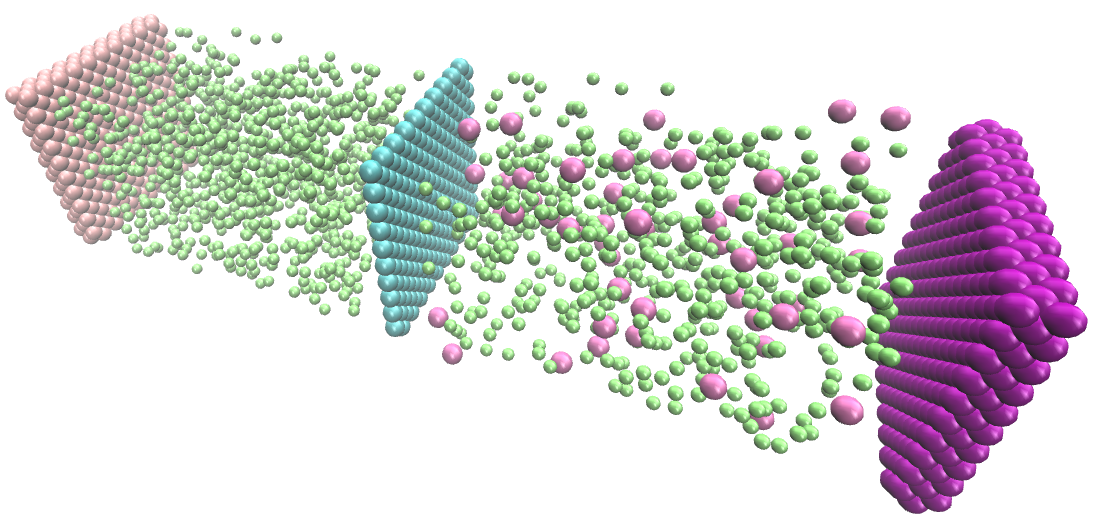
\includegraphics[width=7cm]{media/004-permeable-membrane-minimized.png}
\hfill
}
\end{frame}

\begin{frame}[fragile]{\secname}
Now we can stablish a solution strategy to tackle the problem:

\vspace{0.5cm}

\begin{enumerate}
\item First we create the system (walls, membrane, place atoms, set their properties) and call the minimization function to get a good starting point.

\item Next we run the simulation starting with minimized state. In this we fix membrane position and apply no forces to the walls, but leave them with a degree of freedom to move over $x$ axis, so that their position finds an equilibrium coordinate.

\item Finally, departing from the last state, we add some porosity to the membrane and simulate the osmotic pressure effect across the membrane.
\end{enumerate}

\vspace{0.5cm}

With that we already know that the project consists of 3 steps, the last 2 sharing most of the problem specification, thus using code snippets might be useful.
\end{frame}

\subsection{Initial minimization}

\begin{frame}[fragile]{\secname}{\subsecname\ - Initialization}
The system is initially not equilibrated. In fact we don't know where to specifically place the walls limiting the fluid.

\vspace{0.5cm}

In \LAMMPS\ this can be overcome with boundary condition type \lammpsInline{s}, which stands for \emph{shrink-wrapped}. With this condition the position of the box faces along are set so as to integrate the atoms in that dimension, no matter how far they move.

\vspace{0.5cm}

Below we apply it to the $x$ direction and also provide a \lammpsInline{lj/cut} cut-off potential.

\vspace{0.5cm}

\begin{lstlisting}[language=LAMMPS,basicstyle=\small]
boundary	 s p p
pair_style	 lj/cut 2.5
\end{lstlisting}
\end{frame}

\begin{frame}[fragile]{\secname}{\subsecname\ - Lattice creation}
To create the solid elements we need to specify a \lammpsDocs{lattice} prior to creating the region. There will be \lammpsInline{5} atom types in this simulation, one for each solid and two fluid species.

\vspace{0.5cm}

\begin{lstlisting}[language=LAMMPS,basicstyle=\small]
lattice       fcc 1
region        domain block  -23  23  -5  5  -5  5
create_box    5 domain
\end{lstlisting}
\end{frame}

\begin{frame}[fragile]{\secname}{\subsecname\ - Named regions}
As usual, its is practical to provided named regions.

\vspace{0.5cm}

Notice that they are unbounded in both $y$ and $z$ directions.

\vspace{0.5cm}

\begin{lstlisting}[language=LAMMPS,basicstyle=\tiny]
region        piston_left   block  -21.00  -20.00  INF  INF  INF  INF
region        fluid_left    block  -18.00   -2.00  INF  INF  INF  INF
region        membrane      block   -0.25    0.25  INF  INF  INF  INF
region        fluid_right   block    2.00   18.00  INF  INF  INF  INF
region        piston_right  block   20.00   21.00  INF  INF  INF  INF
\end{lstlisting}
\end{frame}

\begin{frame}[fragile]{\secname}{\subsecname\ - Filling the system}
If atoms are created in a region, they will occupy the lattice defined there.
Randomly placed atoms will form the fluid. It is this subtle difference that will define what atoms belong to each phase.

\vspace{0.5cm}

Notice that atom type \lammpsInline{4} (solvent) is used in both left and right fluids.

\vspace{0.5cm}

\begin{lstlisting}[language=LAMMPS,basicstyle=\tiny]
# Add atoms to what will be solid.
create_atoms  1 region piston_left
create_atoms  2 region membrane
create_atoms  3 region piston_right

# Add atoms to what will be fluid.
create_atoms  4 random 1000 654514  fluid_left
create_atoms  4 random 550  654514  fluid_right
create_atoms  5 random 50   424514  fluid_right
\end{lstlisting}
\end{frame}

\begin{frame}[fragile]{\secname}{\subsecname\ - Usage of wildcards}
If you have some experience with command line or scripting (and you should have some for managing your MD projects), you probably know what are \emph{wildcards}. \LAMMPS\ provides some support to them, but sometimes in unusual ways.

\vspace{0.5cm}

Below we set the mass of all atoms to unity by placing a star \lammpsInline{*} in place of atom indexes (what agrees with its usage in most \emph{nix} systems).

\vspace{0.5cm}

\begin{lstlisting}[language=LAMMPS,basicstyle=\small]
mass          * 1.0
\end{lstlisting}
\end{frame}

\begin{frame}[fragile]{\secname}{\subsecname\ - More on wildcards}
It is not always that \LAMMPS\ wildcard convention will match the typical. In the following snippet, the use of \lammpsInline{1*3  1*3} implies all pairwise combinations between atoms of types 1 to 3.

\vspace{0.5cm}

\begin{lstlisting}[language=LAMMPS,basicstyle=\small]
# Pair-wise coefficients.
pair_coeff    1*3  1*3  1.0  1.0
pair_coeff    4    4    1.0  1.0
pair_coeff    5    5    2.0  3.0
\end{lstlisting}

\vspace{0.5cm}

To confirm this, check section \Verb|PairIJ Coeffs| of restart file generated after running the first step of this tutorial.
\end{frame}

\begin{frame}[fragile]{\secname}{\subsecname\ - Overriding defaults}
We already discussed how \LAMMPS\ handles pair coefficients for interactions between atoms of different types. You can also enforce the values to take any user-defined values (and in more advanced cases, models).

\vspace{0.5cm}

Below we make interaction between solids and solvent \lammpsInline{4} / solute \lammpsInline{5} weaker, and also set the size of solute \lammpsInline{5} to a higher value to make membrane traversal less likely.

\vspace{0.5cm}

\begin{lstlisting}[language=LAMMPS,basicstyle=\small]
# Impose dissimetric coefficients for walls and solvent/solute.
pair_coeff    1*3  4    0.8  1.0
pair_coeff    1*3  5    0.1  3.0
\end{lstlisting}
\end{frame}

\begin{frame}[fragile]{\secname}{\subsecname\ - Run minimization}
This concludes the basic initialization and we can run the energy minimization followed by dump of restart file for what comes next.

\vspace{0.5cm}

\begin{lstlisting}[language=LAMMPS,basicstyle=\small]
thermo        10
minimize      1.0e-04  1.0e-06  1000  10000
write_data    "dumps/step-1-restart.min.lammps" pair ij
\end{lstlisting}
\end{frame}

\subsection{System equilibration}

\begin{frame}[fragile]{\secname}{\subsecname\ - Restarting from state}
By now you should be familiar with restarting a simulation from a dumped state. The following snipped illustrates how succinct it can be with use of included files, discussed in the next slides.

\vspace{0.5cm}

\begin{lstlisting}[language=LAMMPS,basicstyle=\tiny]
# Initialization -------------------------------------------------------------

include       "config/01-initialize.lammps"

# System definition ----------------------------------------------------------

read_data     "dumps/step-1-restart.min.lammps"
include       "config/02-system-definition.lammps"

# Simulation settings --------------------------------------------------------

include       "config/03-simulation-settings.lammps"
\end{lstlisting}
\end{frame}

\begin{frame}[fragile]{\secname}{\subsecname\ - Creating groups}
File \Verb|config/02-system-definition.lammps| is provided below. It simply provides groups for atom manipulations in upcoming steps.

\vspace{0.5cm}

The first \lammpsInline{neigh_modify} call is not necessary but will improve simulation performance by excluding the interactions between solid-solid atoms from updates of neighbor lists.

\vspace{0.5cm}

\begin{lstlisting}[language=LAMMPS,basicstyle=\tiny]
# Create region on right side of membrane for recording fluxes.
region       right block 0 INF INF INF INF INF

group        solid        type 1 2 3
group        fluid        type 4 5

group        piston_left  type 1
group        membrane     type 2
group        piston_right type 3
group        solvent      type 4
group        solute       type 5

neigh_modify exclude group solid solid
neigh_modify every 1 delay 5 check yes
\end{lstlisting}
\end{frame}

\begin{frame}[fragile]{\secname}{\subsecname\ - Simulation settings}
Simulation settings are shared by the initial equilibration being discussed here and the next step, the simulation run. You can check the contents of the included snippet file \href{https://github.com/WallyTutor/learning-scientific-computing/blob/main/molecular-dynamics/lammps/tutorials-simon-gravelle/02-Permeable-Membrane/config/03-simulation-settings.lammps}{\Verb|config/03-simulation-settings.lammps|} on the repository .

\vspace{0.5cm}

The only point I would like to discuss further here is the different between providing zero force or \lammpsInline{NULL}, the latter leaving a movement degree of freedom.

\vspace{0.5cm}

\begin{lstlisting}[language=LAMMPS,basicstyle=\tiny]
# Cancel forces on membrane to keep it fixed.
fix           mysf1 membrane setforce 0 0 0

# Freeze pistons but allow movement over x with NULL (leave a DoF).
fix           mysf2 piston_left  setforce NULL 0 0
fix           mysf3 piston_right setforce NULL 0 0
\end{lstlisting}
\end{frame}

\begin{frame}[fragile]{\secname}{\subsecname\ - Run equilibration}
To conclude this step, we add a few fixes to keep track of concentrations and piston positions. Simulation is run for a large number of steps aiming at initial equilibration.

\vspace{0.5cm}

\begin{lstlisting}[language=LAMMPS,basicstyle=\tiny]
fix           myat1 all ave/time 1000 1 1000 v_solvent_right         &
               file "dumps/step-2-solvent-right.dat"
fix           myat2 all ave/time 1000 1 1000 v_solute_right          &
               file "dumps/step-2-solute-right.dat"
fix           myat3 all ave/time 1000 1 1000 v_position_piston_left  &
               file "dumps/step-2-position-piston-left.dat"
fix           myat4 all ave/time 1000 1 1000 v_position_piston_right &
               file "dumps/step-2-position-piston-right.dat"

dump          mydmp all atom 1000 &
              "dumps/step-2-dynamics.lammpstrj"

thermo_modify temp temperature_fluid

# Run simulation -------------------------------------------------------------

thermo        10000
run           500000
write_data    "dumps/step-2-restart.min.lammps" pair ij
\end{lstlisting}
\end{frame}

\begin{frame}[fragile]{\secname}{\subsecname\ - Convergence check}
Before going further towards production run, we verify the pistons have found an equilibrium position, as illustrated below. This validates the initialization and we can advance to next steps.

\vspace{0.5cm}

{%
\hfill
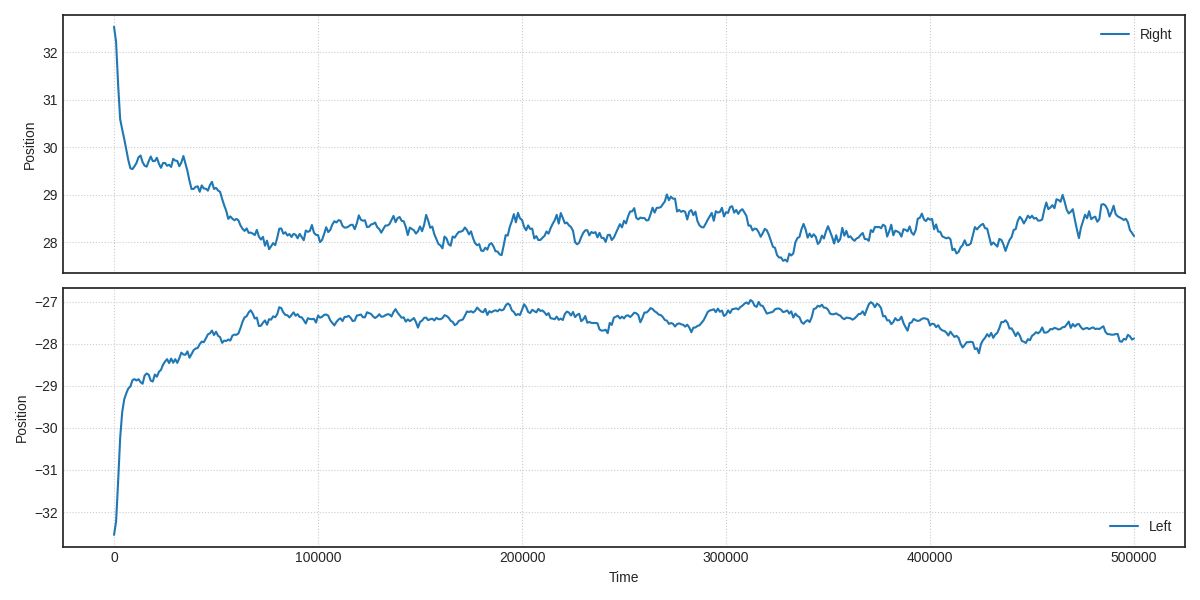
\includegraphics[width=8cm]{media/005-permeable-membrane-piston-position.png}
\hfill
}
\end{frame}

\subsection{Production run}

\begin{frame}[fragile]{\secname}{\subsecname\ - Making membrane porous}
Final script can be found \href{https://github.com/WallyTutor/learning-scientific-computing/blob/main/molecular-dynamics/lammps/tutorials-simon-gravelle/02-Permeable-Membrane/input-step-3.lammps}{here}. The only difference with regards to the system equilibration we just performed is the random deletion some atoms from the membrane, so that it is porous.

\vspace{0.5cm}

In newer versions of \LAMMPS\ you can delete the last 2 lines and comment out the second line of the following snippet.

\vspace{0.5cm}

\begin{lstlisting}[language=LAMMPS,basicstyle=\small]
# Delete 50% of atoms from membrane.
# delete_atoms random fraction 0.5 no all membrane 482793
region       membrane block -0.25 0.25 INF INF INF INF
delete_atoms porosity membrane 0.5 482793
\end{lstlisting}
\end{frame}

\begin{frame}[fragile]{\secname}{\subsecname\ - Final results}
If everything went well you probably got results similar to the following. With that we are ready to go to the next step!

\vspace{0.5cm}

{%
\hfill
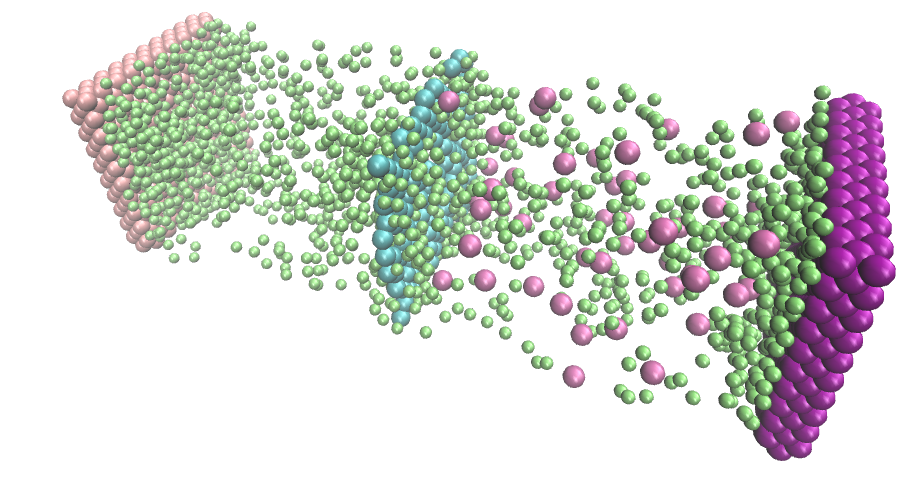
\includegraphics[width=6cm]{media/006-permeable-membrane-final.png}
\hfill
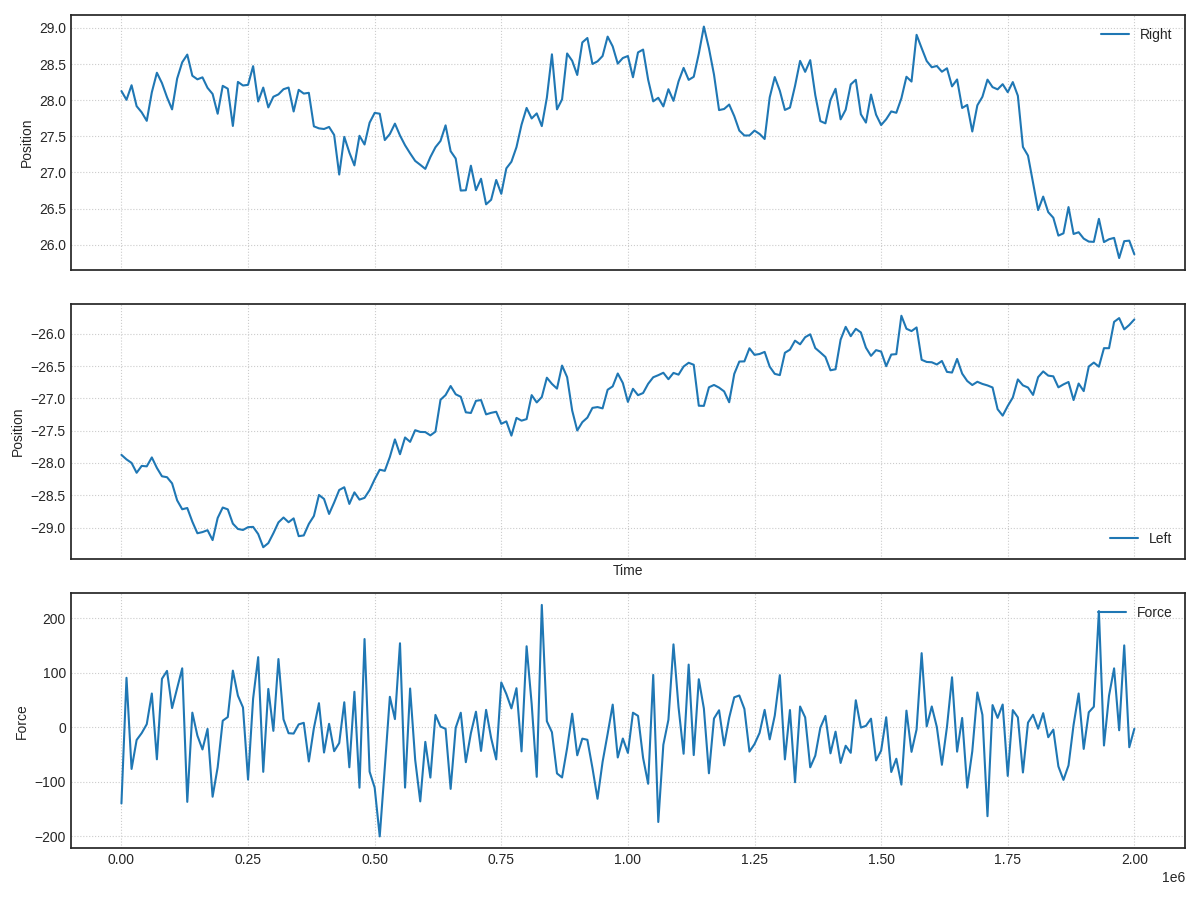
\includegraphics[width=6cm]{media/008-permeable-membrane-piston-position.png}
\hfill
}
\end{frame}

\endinput